\documentclass[english, 11pt]{article}
\usepackage{../notes}
\usepackage{lipsum}

%Global Course Variables
\newcommand{\myCourseCode}{EECS 445}
\newcommand{\myCourseName}{Introduction to Machine Learning}
\newcommand{\myProf}{Honglak Lee}
\newcommand{\myTerm}{Fall 2015}

%Headers
\lhead{\myCourseName}
\rhead{\fancyplain{}{\rightmark}} 

%Footers
\cfoot{\thepage}

\begin{document}
\titleHeader{\myCourseCode}{\myCourseName}{\myProf}{\myTerm}

%Document information
\rule{1\columnwidth}{.5pt}
Contributors: Max Smith
\begin{center}
	Latest revision: \today
\end{center}
\toc
\abstr{Theory and implementation of state-of-the-art machine learning algorithms for large-scale real-world applications. Topics include supervised learning (regression, classification, kernel methods, neural networks, and regularization) and unsupervised learning (clustering, density estimation, and dimensionality reduction).}

%----------------------------
%Document Begins
%----------------------------
% Unnamed Examples:

\begin{defn}
	A relative path is a path that is referring to your current directory.
\end{defn}

\begin{rem}
	Recall that double quotes do not protect back quotes.
\end{rem}

\begin{exmp}
	$$2+2=3$$
\end{exmp}

With some names:
\begin{defn}[Relative Path]
    A relative path is a path that is referring to your current directory.
\end{defn}

\begin{rem}[Double Quotes]
    Recall that double quotes do not protect back quotes.
\end{rem}

\begin{exmp}[Addition]
    $$2+2=3$$
\end{exmp}

\section{Readings}
	\subsection{Probability Distributions}
	\begin{defn}[Binary Variable]
	Single variable that can take on either 1, or 0; $x\in \{0, 1\}$. We denote $\mu$ ($0\leq\mu\leq 1$) to be the probability that the random binary variable $x=1$
	$$p(x=1|\mu)=\mu$$
	$$p(x=0|\mu)=1-\mu$$
\end{defn}

\begin{defn}[Bernoulli Distribution]
	Probability distribution of the binary variable x, where $\mu$ is the probability $x=1$.
	$$\text{Bern}(x|\mu)=\mu^x(1-\mu)^{1-x}$$
	The distribution has the following properties:
	\begin{itemize}
		\item $\text{E}(x)=\mu$
		\item $\text{Var}(x)=\mu (1-\mu)$
		\item $\mathcal{D}=\{x_1,\ldots ,x_N\} \to p(\mathcal{D} | \mu )=\Pi_{n=1}^{N}p(x_n|\mu)$
		\item Maximum likelihood estimator: $\mu_{ML}=\frac{1}{N}\sum_{n=1}^{N}x_n=\frac{numOfOnes}{sampleSize}$ (aka. sample mean)
	\end{itemize}
\end{defn}

\begin{defn}[Binomial Distribution]
	Distribution of $m$ observations of $x=1$, given a sample size of $N$. 
	$$\text{Bin} (m|N,\mu={\substack{N\\m}}\mu^m (1-\mu )^{N-m}$$\
	\begin{itemize}
		\item $\text{E}(m)=N\mu$
		\item $\text{Var}(m)=N\mu (1-\mu )$
	\end{itemize}
\end{defn}

\subsubsection{The Beta Distribution}
In order to develop a Bayesian treatment for fitting data sets, we will introduce a prior distribution $p(\mu)$.

\begin{itemize}[--]
	\item \textbf{Conjugacy:} when the prior and posterior distributions belong to the same family.
\end{itemize}

\begin{defn}[Beta Distribution]
	$$\text{Beta}(\mu |a,b)=\frac{\Gamma (a+b)}{\Gamma (a)\Gamma (b)}\mu^{a-1} (1-\mu )^{b-1}$$
	Where $\Gamma (x)$ is the gamma function.
	The distribution has the following properties:
	\begin{itemize}
		\item $\text{E}(\mu )=\frac{a}{a+b}$
		\item $\text{Var}(\mu )=\frac{ab}{(a+b)^2 (a+b+1)}$
		\item conjugacy
		\item ${a\to\infty || b\to\infty}\to \text{variance}\\to 0$ 
	\end{itemize}

	Conjugacy can be shown by the distribution by the likelihood function (binomial):
	$$p(\mu |m,l,a,b)\propto \mu^{m+a-1} (1-\mu )^{l+b-1}$$
	Normalized to:
	$$p(\mu |m,l,a,b)= \frac{\Gamma (m+a+l+b)}{\Gamma (m+a)\Gamma (l+b)} \mu^{m+a-1} (1-\mu )^{l+b-1}$$
\end{defn}

\begin{itemize}[--]
	\item \textbf{Hyperparameters:} parameters that control the distribution of the regular parameters.
	\item \textbf{Sequential Approach:} method of learning where you make use of an observation one at a time, or in small batches, and then discard them before the next observatiosn are used. (Can be shown with a Beta, where observing $x=1\to a++, x=0\to b++$, then normalizing)
	\item For a finite data set, the posterior mean for $\mu$ always lies between the prior mean and the maximum likelihood estimate.
	\item A general property of Bayesian learning is when we observe more and more data the uncertainty of the posterior distribution will steadily decrease.
	\item More information and examples of probability distributions can be found in Appendix B of Bishop's `Pattern Recognition and Machine Learning.'
\end{itemize}


	\subsection{Linear Models for Regression}
	\begin{itemize}[--]
	\item \textbf{Linear Regression:} $y(\mathbf{x}, \mathbf{w})=w_0+w_1 x_1+\ldots +w_D x_D$
	\item Limited on linear function of input variables $x_i$
	\item Extend the model with nonlinear functions, where $\phi_j (x)$ are known as basis functions:
		$$y(\mathbf{x}, \mathbf{w})=w_0 +\sum_{j=1}^{M-1}w_j\phi_j (x)$$
	\item $w_0$ allows for any fixed offset in data, and is known as the \textbf{bias parameter}.
	\item Given a dummy variable $\phi_0 (x)=1$, our model becomes:
		$$y(\mathbf{x}, \mathbf{w})=\sum_{j=0}^{M-1}w_j\phi_j (x)=\mathbf{W}^\mathbf{T} \mathbf{\phi} (x)$$
	\item Functions of this form are called \textbf{linear models} because the function is linear in weight.
\end{itemize}

\subsubsection{Maximum likelihood and least squares}
\begin{itemize}[--]
	\item j
\end{itemize}

\section{Stanford Notes}
	\subsection{Linear Regression with One Variable}
	\subsubsection{Model Representation}
\begin{itemize}[--]
	\item Goal is model labelled data (data which we have the correct output for) to a line 
	\item Notation:\begin{description}
		\item[$m$] = number of training examples
		\item[$x$] = input variable/feature
		\item[$y$] = output variable/feature
		\item[$(x,y)$] = one training example
		\item[$(x^{(i)},y^{(i)})$] = $i$th training example (parens indicate index)
	\end{description}

	\item We take a training set, input into a learning algorithm, which returns a hypothesis ($h$) that models the relationship.
	\begin{center}\begin{tikzpicture}[node distance = 2cm, auto]
		%Place nodes
		\node [block] (train) {Training Set};
		\node [block, below of=train] (alg) {Learning Algorithm};
		\node [block, below of=alg] (hyp) {$h$};
		\node [cloud, left of=hyp] (x) {$x$};
		\node [cloud, right of=hyp] (y) {$y$};

		%Draw edges
		\path [line] (train) -- (alg);
		\path [line] (alg) -- (hyp);
		\path [line] (x) -- (hyp);
		\path [line] (hyp) -- (y);
	\end{tikzpicture}\end{center}
	\item $h$ maps from $x$'s to $y$'s ($h(x)=y$).
	\item We need to determine how we want to represent $h$
	\item A simple linear model with one variable for $h$ is: $$h_\theta (x) = \theta_0 + \theta_1 x$$, called \textbf{univariate linear regression}.
\end{itemize}

\subsubsection{Cost Function}
\begin{itemize}[--]
	\item Given a hypothesis: $h_\theta (x) = \theta_0 + \theta_1 x$
	\begin{description}
		\item[$\theta_i's$] = parameters of the model
	\end{description}

	\item We will now discuss how to choose the parameters of our model
	\item Idea: choose $\theta_0, \theta_1$ so that $h_\theta (x)$ is close to $y$ for our training examples $(x,y)$
	\item We want to minimize $\theta_0, \theta_1$ such that $h(x) - y$ is minimal (reminder: $h(x)$ is the guess at the correct value at $y$).
	\item Because we we only are looking to minimize our absolute distance, we square the distance we want to minimize to account for positive and negative differences equally now making our cost function: $(h(x)-y)^2$
	\item However, we don't want to minimize it for just one example, so we do this for every training example: $$\sum_{i=1}^{m}(h_\theta (x^{(i)}) - y^{(i)})^2$$
	\item To make later math easier, we further refine our formula to be half the average: $$\frac{1}{2m}\sum_{i=1}^{m}(h_\theta (x^{(i)}) - y^{(i)})^2$$
	\item This function we created is called our \textbf{cost} function, as it measures how expensively incorrect our current model is, which we will denote with $J$. 
	\item The cost function is dependent on the hypothesis parameters, and our goal is to adjust these parameters to minimize the overrall cost of our model: $$J(\theta_0, \theta_1) = \frac{1}{2m}\sum_{i=1}^{m}(h_\theta (x^{(i)}) - y^{(i)})^2$$
	\item Now our goal is to minimize $J$ over the variables $\theta_0, \theta_1$
\end{itemize}

\subsubsection{Cost Function - Intuition I}
\begin{center}
	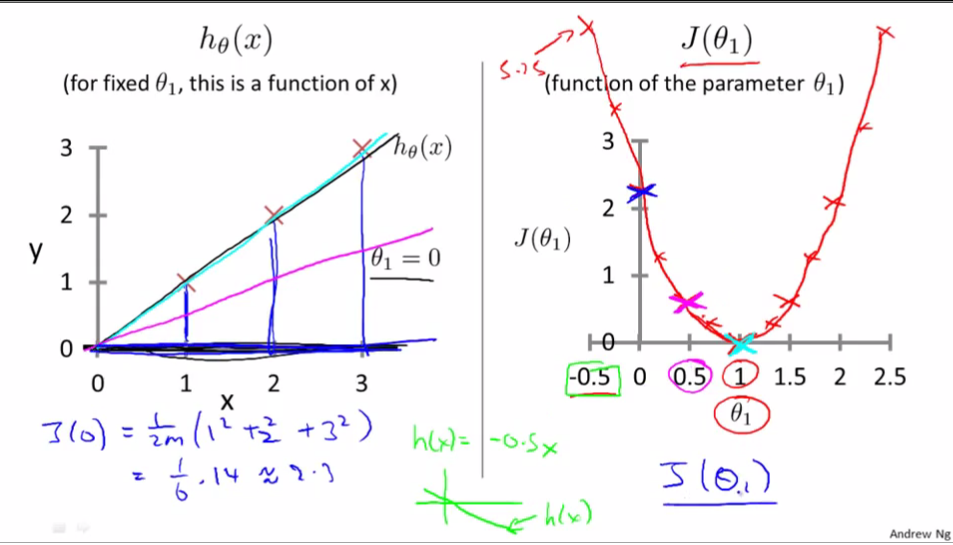
\includegraphics[scale=0.75]{sections/cs229/w1/cost_function.png}
\end{center}
This image shows that for varying parameter values, the cost function changes. In this idealistic example there's a global minimum, the goal of minimized cost, that is very easily followed by a hill-climbing style algorithm.

\subsubsection{Cost Function - Intuition II}
\begin{center}
	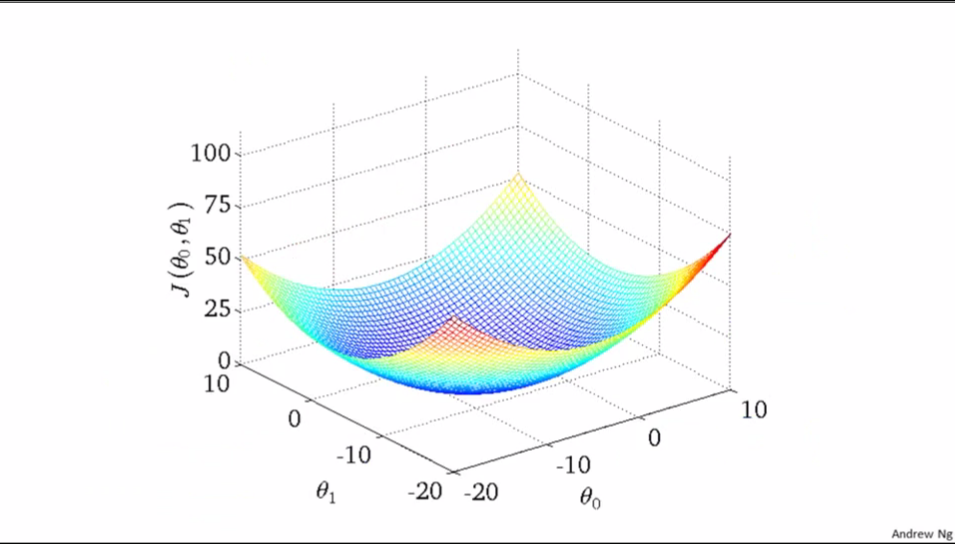
\includegraphics[scale=0.75]{sections/cs229/w1/2d_cost_function.png}
\end{center}
Similarly when you have an additional variable, you want to reach the bottom of this $N$-dimensional hill (note: not all models will have such a perfect hill). 
\begin{itemize}[--]
	\item The gradient gives the direction of maximumal increase on a surface.
	\item We will use a negative gradient to find the `direction' to travel towards the bottom of the hill
	\item Another common way to represent multidimensional cost functions is through contour plots
	\item 
\end{itemize}

	\subsection{Linear Regression with Multiple Variables}
	\subsubsection{Multiple Features}
\begin{itemize}[--]
	\item Instead of just one feature ($x$), we known multiple features ($x_1,\ldots, x_n$). eg. size, number of bedrooms, number of floors, age of home.
	\item $x^{(i)}_j:$ value of feature $j$ in $i^{th}$ training example
	\item Now our hypothesis must account for multiple features: 
		$$h_\theta (x)=\theta_0 + \theta_1 x_1 + \ldots \theta_n x_n$$
	\item Again we define $x_0 = 1$ to simplify future math ($x^{(i)}_0=1$).
	$$x=\begin{bmatrix} x_1\\ \vdots\\ x_n\end{bmatrix}\in \mathbb{R}^{n+1}\text{,  }
		\theta = \begin{bmatrix}\theta_0 \\ \vdots\\ \theta_n\end{bmatrix}\in\mathbb{R}^{n+1}$$
	\item Transposing the $\theta$ vector given our assumption for $x_0^{(i)}$ allows us to simplify our hypothesis into:
		$$h_\theta (x) = \theta^{T}x$$
\end{itemize}

\subsubsection{Gradient Descent for Multiple Variables}
\begin{itemize}[--]
	\item Repeat until convergence ($j=0,\ldots, n$): 
		$$\theta_j := \theta_j \alpha\frac{1}{m}\sum_{i=1}^{m}(h(x^{(i)}-y^{(i)}))x^{(i)}_j$$
	\item This is a valid generalization of the previous formula because of our base case $x^{(i)}_0=1$
\end{itemize}

\subsubsection{Gradient Descent in Practice I - Featuer Scaling}
\begin{itemize}[--]
	\item \textbf{Feature scaling:} if features are on similar scales then we converge more quickly
	\item Your parameters will oscillate along the larger ranged parameter making it's way much slower towards the center (in the case of two variables); whereas, if both axis were equal then you don't have a worst case to fret about
	\begin{center}
		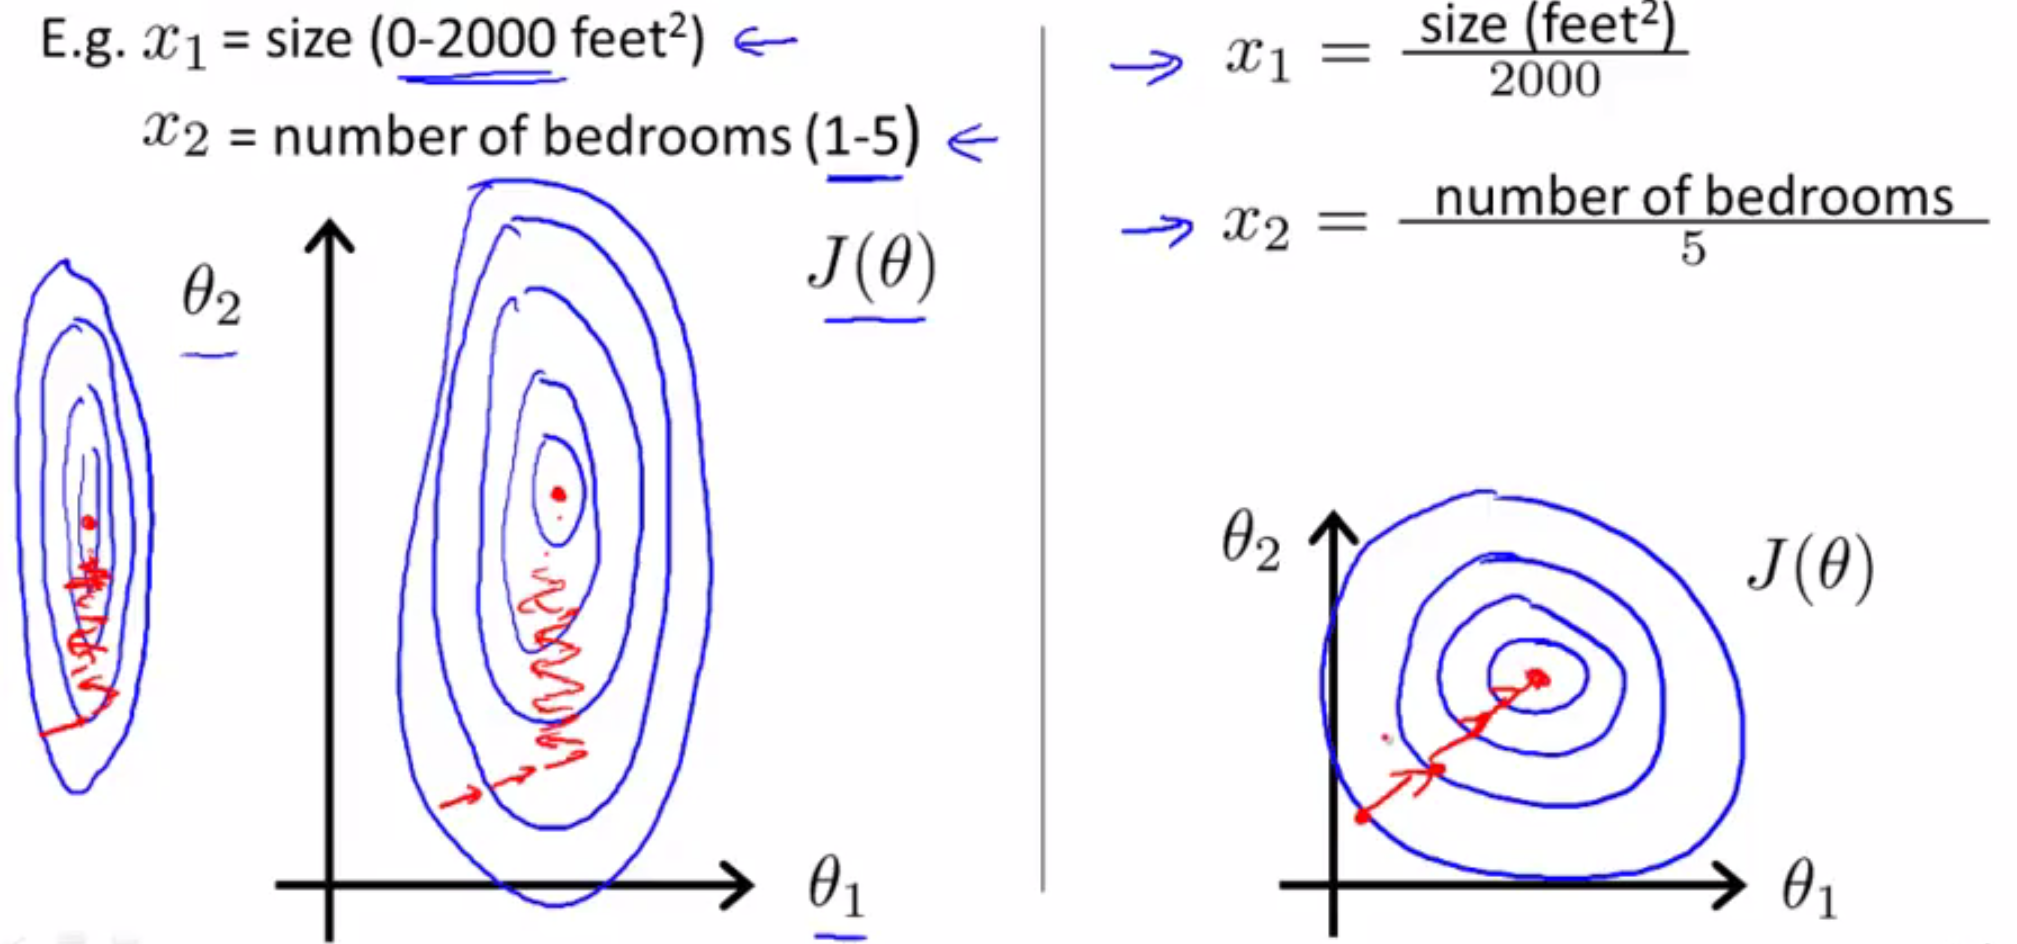
\includegraphics[scale=0.25]{sections/cs229/w2/feature_scaling.png}
	\end{center}

	\item Typically, we want to scale each feature into approximately a $-1\leq x_i \leq 1$ range (same order of magnitude).
	\item \textbf{Mean normalization:} replacing $x_i$ with $x_i-\mu_i$ to make features have approximately zero mean (does not apply to $x_0=1$).
	\item Combining mean normalization and feature scaling we assign $x_i := \frac{x_i-\mu_i}{range_i}$

\end{itemize}

\subsubsection{Gradient Descent in Practice II - Learning Rate}
\begin{itemize}[--]
	\item To ensure gradient descent is working correctly, plot the cost function against the number of iterations. It should converge towards 0, decreasing at every iteration.
	\item The number of iterations required can vary widely for different applications
	\item You can create an automatic convergence test to ensure appropriately ending of gradient descent by checking if the difference between two iterations $\epsilon$ is below a threshold.
	\item If there is any increase in slope, use a smaller $\alpha$
	\item For sufficiently small $\alpha$, $J(\theta )$ should decrease on every iteration
	\item But if $\alpha$ is too small, gradient descent an be slow to converge
	\item To choose $\alpha$ try: $\ldots, 0.001, 0.003, 0.01, 0.03, 0.1, 0.3, 1,\ldots$
\end{itemize}

\subsubsection{Features and Polynomial Regression}
\begin{itemize}[--]
	\item Suppose we have a housing price prediction: $h(x)=\theta_0 + \theta_1 (frontage)+\theta_2 (depth)$
	\item We can define a new feature $(area)=(frontage)(depth)$, that we can use in a new hypothesis $h(x)=\theta_0+\theta_1 (area)$
	\item We can map these hypothesis of more complex features into a linear regression problem: 
	\begin{align*}
		h(x)&=\theta_0 + \theta_1 x_1 + \theta_2 x_2 + \theta_3 x_3    
  		  	&=\theta_0 + \theta_1 (size) + \theta_2 (size)^2 + \theta_3 (size)^3
	\end{align*}

	\item If your features are like those chosen, then feature scaling is very important
	\item There are many more choices for modifications to our features (such as: $\sqrt{}$).
	\item Trying new features can allow you to have a more appropriate model
\end{itemize}

\subsubsection{Normal Equations}
\begin{itemize}[--]
	\item The \textbf{normal equation} allows us to solve for $\theta$ analytically (without iterations)
	\item Intuition: $J(\theta) = a\theta^2+b\theta+c$
	In previous calculus classes you would find the minimum by taking the derivative set equal to 0 and solving for $\theta$. 
	\item This can be extended with partial fractions and solving for every $\theta_j\in\theta$. $$\frac{\partial}{\partial\theta_j}J(\theta)=\ldots=0 \text{    (for every}j\text{)}$$
	\item We construct a matrix from the features and a vector from the solutions as so ($n$ features, $m$ examples):

	\[X=\begin{bmatrix}
		x_0^{(1)} & x_1^{(1)} & \dots & x_n^{(1)} \\
		x_0^{(2)} & x_1^{(2)} & \dots & x_n^{(2)} \\
		\vdots & \vdots & \ddots & \vdots \\
		x_0^{(m)} & x_1^{(m)} & \dots x_n^{(m)} 
	\end{bmatrix} \in \mathbb{R}^{m\times (n+1)}
	 \]

	 \[
	y=\begin{bmatrix}
		y^{(1)} \\
		y^{(2)} \\
		\vdots \\
		y^{(m)}
	\end{bmatrix}\in \mathbb{R}^{m\times 1}
	 \]

	 \item We can then represent the $\theta$ by the \textbf{normal equation} $$\theta = (X^{T}X)^{-1}X^{T}y$$\
	 \item $X$ is entitled the \textbf{design matrix}
	 \item Normal equation does not perform well with a large $n$ due to the computation $(X^{T}X)^{-1}\in\mathbb{n\times n}$ which is typically $\O{n^3}$
\end{itemize}

	\subsection{Logistic Regression}
	\subsubsection{Multiple Features}
\begin{itemize}[--]
	\item 
\end{itemize}


  
	\subsection{Regularization}
	\subsubsection{The Problem of Overfitting}
\begin{itemize}[--]
	\item \textbf{Underfitting}: when a model cannot capture the underlying trend of the data ("high bias")
	\item \textbf{Overfitting}: when a model captures the noise of the data ("high variance")
	\item \textbf{Generalize}: fails to fit to new examples
	\item Overfitting's poor generalization results in low costs not always being correct
	\begin{center}
		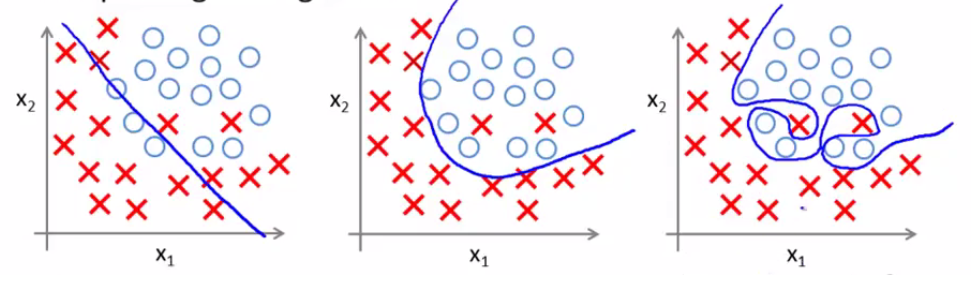
\includegraphics[scale=0.5]{sections/cs229/w4/over-under.png}
	\end{center}

	\item If we have too many features for very little data, overfitting can easily become a big problem.
	\item Options:
	\begin{itemize}
		\item Reduce number of features
		\begin{itemize}
			\item Manually select which features to keep
			\item Model selection algorithm (later in course)
		\end{itemize}
		\item Regularization
		\begin{itemize}
			\item Keep all the features, but reduce magnitude/values of parameters $\theta_j$
			\item Works well when we have a lot of features, each of which contributes a bit to predicting $y$
		\end{itemize}
	\end{itemize}

\end{itemize}

\subsubsection{Cost Function}
\begin{itemize}[--]
	\item Having smaller values for parameters $\theta_0, \theta_1, \ldots, \theta_n$
	\begin{itemize}[--]
		\item ``Simpler'' hypothesis
		\item Less prone to overfitting
	\end{itemize}

	\item To exemplify lets consider the housing scenario:
	\begin{itemize}[--]
		\item Features: $x_1,\ldots, x_100$
		\item Paremeters: $\theta_0, \ldots, \theta_100$
		\item We don't know which ones are complex to shrink, so we modify the cost function to shrink every parameter
		$$J(\theta )=\frac{1}{2m}(\sum_{i=1}^{m}(h(x^{(i)}-y^{(i)})^2 + \lambda\sum_{i=1}^{n}\theta_j^2)$$
		\item We don't penalize $\theta_0$ by convention, because it's a constant and makes very little difference
	\end{itemize}

	\item $\lambda$ is called the regularization parameter. It controls the trade off of fitting the training set well and keeping the parameters small and simple to prevent overfitting
	\item If $\lambda$ is set to be very large we will penalize all the paramters extremely highly resulting which will result in all by the constant being close to zero (fits to a horizontal line). ``Underfit''
\end{itemize}

\subsubsection{Regularized Linear Regression}
\begin{itemize}[--]
	\item Using the new regularized linear regression cost function from the previous section we can now update our gradient descent algorithm to encorporate this modification:
		$$\theta_0 := \theta_0 - \alpha\frac{1}{m}\sum_{i=1}^{m} (h(x^{(i)})-y^{(i)})x_0^{(i)}$$
		$$\theta_j := \theta_j - \alpha ( \frac{1}{m}\sum_{i=1}^{m}(h(x^{(i)})-y{(i)})x)j^{(i)} +\frac{\lambda}{m}\theta_j )$$

	\item The $\theta_j$ $(j=1,\ldots, n)$ term can also be written:
		$$\theta_j := \theta_j (1-\alpha\frac{\lambda}{m}) - \alpha\frac{1}{m}\sum_{i=1}^{m}(h(x^{(i)}) - y^{(i)})x_j^{(i)}$$

	\item The term $(1-\alpha\frac{\lambda}{m})$ is typically $<1$, so this results in shrinking $\theta_j$ by multiplying by a value $<1$, and then performing the same gradient descent function
	\item We also had the normal equation to solve the same problem, and it can also be updated for regularization:
		$$\theta = (X^{T}X+\lambda \left[ \begin{smallmatrix}
			0 & & &\\
			& 1 & &  \\
			& & \ldots & \\
			& & & 1 
		\end{smallmatrix}\right] )X^{T}y$$

	\item Suppose $m\leq n$ then $(X^{T}X)$ will be non-invertible/singular
	\item Regularization will take care of this flaw so long as $\lambda > 0$
\end{itemize}

\subsubsection{Regularized Logistic Regression}
\begin{itemize}[--]
	\item We can also regularize logistic regression in a similar manner
		$$\theta_0 := \theta_0 - \alpha\frac{1}{m}\sum_{i=1}^{m} (h(x^{(i)})-y^{(i)})x_0^{(i)}$$
		$$\theta_j := \theta_j - \alpha ( \frac{1}{m}\sum_{i=1}^{m}(h(x^{(i)})-y{(i)})x)j^{(i)} +\frac{\lambda}{m}\theta_j )$$
		$$h(x)=\frac{1}{1+e^{-\theta^{T}x}}$$
\end{itemize}

	\subsection{Neural Networks: Representation}
	\subsubsection{Non-linear Hypothesis}
\begin{itemize}[--]
	\item Suppose you have a housing classification problem with different features $x_1, \ldots ,x_100$ and if we were to include all quadratic terms for linear classification there would be an enourmous number of terms (~5000 features).
	\item Using linear classifiers has an extremely bad asymptotic complexity (n is typically large)
	\item For example computer vision problems are $\O{n^2}$
	\item Neural networks turn out to be a much better way to solve these style problems
\end{itemize}

\subsubsection{Neurons and the Brain}
\begin{itemize}[--]
	\item Neural networks origins are in algorithms that try to mimic the brain
	\item \textbf{``One learning algorithm hypothesis''}: $x$ cortex can learn whatever is hooked up to it
	\begin{itemize}[--]
		\item Auditory cortex can learn to see
		\item Somatosensory cortex (touch) can learn to see
		\item There is one algorithm that can teach anything to do any function
	\end{itemize}
\end{itemize}

\subsubsection{Model Representation I}
\begin{itemize}[--]
	\item Neural networks work by simulating the neurons in the brain
	\item Has ``input wires'' dendrite
	\item Has ``output wires'' axon
	\item Neuron is a computational unit that takes in inputs and produces an output
	\item Neurons communicate with little spikes of electricity through their axons, which another neuron can receiv with its dendrite
	\item In an artificial neural network we model a neuron as a logistic unit:
	\begin{center}\begin{tikzpicture}[node distance=1cm, auto]
		%Place nodes
		\node (x1) {$x_1$};
		\node [below of=x1] (dots) {$x_2$};
		\node [below of=dots] (xn) {$x_3$};

		\node [cloud, right of=dots] (neuron) {  };

		\node [right of=neuron] (h) {$h_\theta (x)$};

		%Draw edges
		\path [line] (x1) -- (neuron);
		\path [line] (dots) -- (neuron);
		\path [line] (xn) -- (neuron);
		\path [line] (neuron) -- (h);
	\end{tikzpicture}\end{center}

		$$x=\begin{bmatrix} x_0\\ x_1\\ x_2\\ x_3 \end{bmatrix}, \theta=\begin{bmatrix}\theta_0 \\ \theta_1 \\ \theta_2 \\ \theta_3 \end{bmatrix}, h(x)=\frac{1}{1+e^{-\theta^{T}x}}$$

	\begin{itemize}[--]
		\item Here the arrows coming from the $x$ are the input wires
		\item The neuron does the computation
		\item Finally the output comes out
	\end{itemize}

	\item The $x_0$ is called the \textbf{bias unit} and is sometimes omitted because it's constant.
	\item \textbf{Activation function}: defines the output of that node given an input or set of inputs
	\item ``weights'' are synonomous with parameters of the model
	\item Neural networks are groups of neurons strung together

	TODO: Neural Network

	$$a_1^{(2)}=g(\theta_{10}^{(1)}x_0+\theta_{11}^{(1)}x_1+\theta_{12}^{(1)}x_2+\theta_{13}^{(1)}x_3)$$
	$$a_2^{(2)}=g(\theta_{20}^{(1)}x_0+\theta_{21}^{(1)}x_1+\theta_{22}^{(1)}x_2+\theta_{23}^{(1)}x_3)$$
	$$a_3^{(2)}=g(\theta_{30}^{(1)}x_0+\theta_{31}^{(1)}x_1+\theta_{32}^{(1)}x_2+\theta_{33}^{(1)}x_3)$$
	$$h(x)=g(\theta_{10}^{(2)}a_0^{(2)}+\theta_{11}^{(2)}a_1^{(2)}+\theta_{12}^{(2)}a_2^{(2)}+\theta_{13}^{(2)}a_3^{(2)})$$

	\item \textbf{Input layer}: first layer of inputted values
	\item \textbf{Output layer}: the final layer that calculates the output value
	\item \textbf{Hidden layer}: the center layers that don't have known outputs (not input or output layer)
	\item $a_i^{(j)}=$ ``activation'' of unit $i$ in layer $j$
	\item $\theta^{(j)}=$ matrix of weights controlling function mapping from layer $j$ to layer $j+1$
	\item If a network has $s_j$ units in layer $j$, $s_{j+1}$ units in layer $j+1$, then $\theta^{(j)}$ will be of dimension $s_{j+1}\times (s_j + 1)$
\end{itemize}

\subsubsection{Model Representation II}
\begin{itemize}[--]
	\item Consider the previous neural network, where we performed the 4 large equations to calculate the output; we will modify the notation to be of the form:
		$$a_1^{(2)}=g(z_1^{(2)})$$
		$$a_2^{(2)}=g(z_2^{(2)})$$
		$$a_3^{(2)}=g(z_3^{(2)})$$
	\item Let us define:
		$$x=\begin{bmatrix}
			x_0 \\ x_1 \\ x_2 \\ x_3
		\end{bmatrix}, z^{(2)}=\begin{bmatrix}
			z^{(2)}_1 \\ z^{(2)}_2 \\ z^{(2)}_3
		\end{bmatrix}$$
	\item This allows us to perform vectorized calculations:
		$$z^{(2)}=\theta^{(1)}x$$
		$$a^{(2)}=g(z^{(2)})$$
	\item If we instead consider the input layers to be the first layer of activation $a^{(1)}=x$, we may redefine our formulas:
		$$z^{(2)}=\theta^{(1)}a^{(1)}$$
		$$a^{(2)}=g(z^{(2)})$$
	\item We can account for any bias units by including $a_0^{(k)}=1$
		$$h(x)=a^{(3)}=g(z^{(3)})=g(\theta^{(2)}a^{(2)})$$
	\item \textbf{Forward propagation}: information only moves in one direction, forward, from the input nodes, through the hidden nodes (if any) and to the output nodes
	\item If you cover part of the neural network, only showing the last two layers, you'll notice that it's just logistic regression
	\item However instead of using the original features $x_1, \ldots, x_n$, they're using the new features it learned on its own $a_1, \ldots, a_n$
	\item This allows you to use better features than if you were constrained to only your own features, the network has the ability to learn any new features it wants
	\item The \textbf{network architecture} is how the neurons are laid out and connected
\end{itemize}

\subsubsection{Examples and Intuitions I}
\begin{itemize}[--]
	\item Non-linear classification example: XOR/XNOR, is difficult to to model

	TODO Graph

	\item For example we can model simple logical operations with logistic regression:
	\begin{center}
		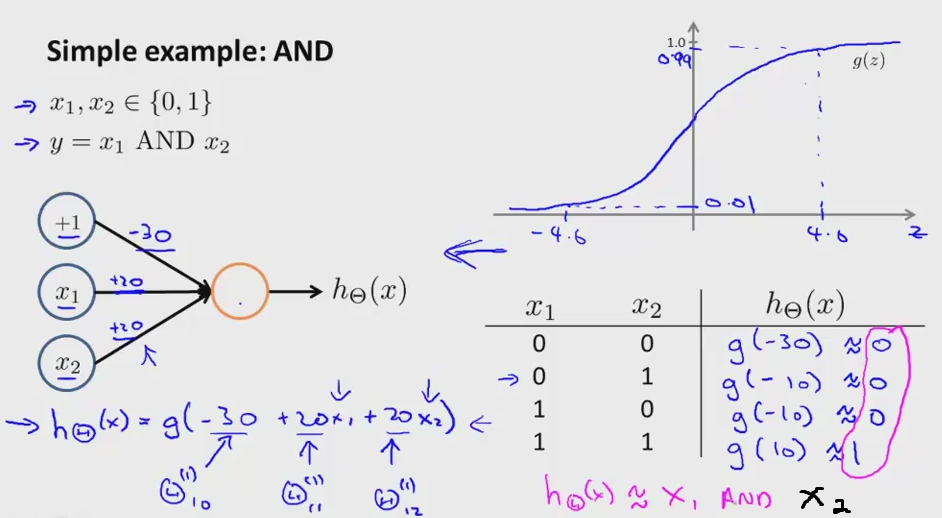
\includegraphics[scale=0.5]{sections/cs229/w5/and_nn.png}
	\end{center}

	\begin{center}
		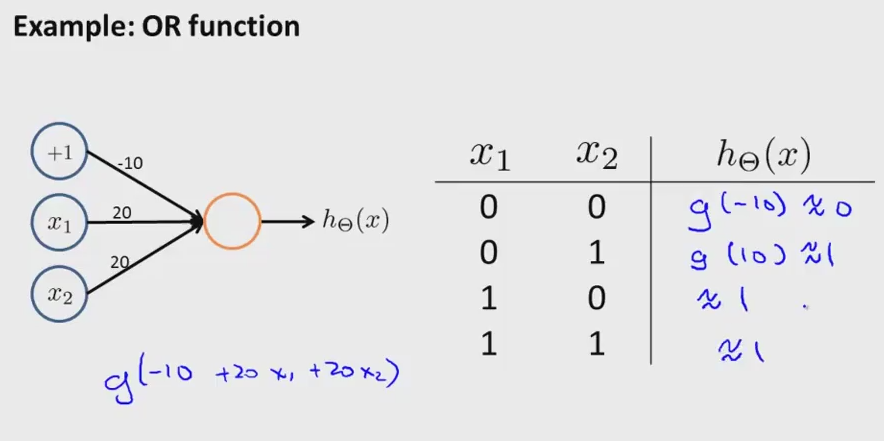
\includegraphics[scale=0.5]{sections/cs229/w5/or_nn.png}
	\end{center}
\end{itemize}

\subsubsection{Examples and Intuitions II}
\begin{itemize}[--]
	\item For models that have non linear boundaries, using a multi-layered network is the best way to approximate the model, for example:
	\begin{center}
		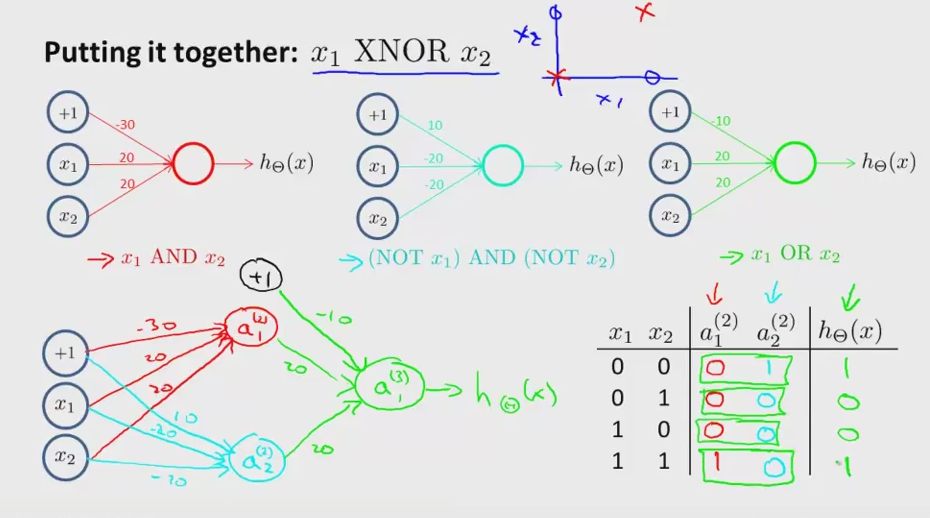
\includegraphics[scale=0.5]{sections/cs229/w5/xnor_nn.png}
	\end{center}

	\item Each layer of the neural network is able to compute even more complex features
	\item The last layer makes the prediction about the correct classification
\end{itemize}

\subsubsection{Multiclass Classification}
\begin{itemize}[--]
	\item Multiclassification is an extension of a one-vs-all 
	\item We want to have the same output units as classes $h(x)\in\mathbb{R}^k$
	\item Each is a classifier for each class, ie. Is it a `1,' is it a `2,' etc..
	\item 
\end{itemize}

	\subsection{Neural Networks: Learning}
	\subsubsection{Cost Function}
\begin{itemize}[--]
	\item Suppose we have:
	\begin{itemize}[--]
		\item Training sets: $\left\{ (x^{(1)}, y^{(1)}),\ldots, (x^{(m)}, y^{(m)})  \right\}$
		\item $m=$ number of training examples
		\item $L=$ total number of layers in network
		\item $s_l=$ number of units (not counting bias unit) in layer $l$
		\item $k=$ number of classes
	\end{itemize}

	\item Binary Classification:
	\begin{itemize}[--]
		\item $y=0\text{ or } 1$
		\item 1 output unit $h(x)\in\mathbb{R}$
		\item $s_l=1$
		\item $k=1$
	\end{itemize}

	\item Multi-class Classification ($K$ classes)
	\begin{itemize}[--]
		\item $y\in\mathbb{R}^K$
		\item $K$ output units
		\item $h(x)\in\mathbb{R}^K$
		\item $s_l=K, (K\geq 3)$
	\end{itemize}

	\item New cost function:
		$$h_{\Theta}(x)\in\mathbb{R}^K, (h_{\Theta}(x))_i=i^{\text{th}}\text{ output}$$
		$$J(\Theta)=-\frac{1}{m}\left[
			\sum_{i=1}^{m}\sum_{k=1}^{K} y_k^{(i)}\log (h(x^{(i)}))_k + (1-y_k^{(i)})\log (1- h(x^{(i)})_k)
			\right] + \frac{\lambda}{2m}\sum_{l=1}^{L-1}\sum_{i=1}^{s_l}\sum_{j=1}^{s_l + 1} (\Theta_{ji}^{(l)})^2$$
\end{itemize}

\subsubsection{Backpropagation Algorithm}
\begin{itemize}[--]
	\item In order to perform gradient descent we need to compute $J(\Theta), \frac{\partial}{\partial\Theta_{ij}}^{(l)} J(\Theta)$
	\item We have already defined $J(\Theta)$, so we just need the partial derivatives.
	\item Intuition: $\delta_j^{(l)}=$ ``error'' of node $j$ in layer $l$
	\item An example is for each output unit (layer $L=4$): $\delta_{j}^{(4)}=a_{j}^{(4)} - y_{j}$
	\item We will comput the $\delta$ for every layer of the neural network
		$$\delta^{(n)} = (\Theta^{(3)})^{T}\delta^{(n+1)} .\times g'(z^{(n)})$$
	\item Where $.\times$ is element-wise multiplication
	\item There is no erro associated with the input layer
	\item The name backpropagation, comes from calculating the error from the back towards the beginning of the network

	\item Suppose we have a training set of $m$ examples
	\item We will set $\Delta_{ij}^{(l)}=0$ (for all $l,i,j$)
	\item This will be used to compute the partial derivatives of the cost function

	TODO: turn into pseudocode

	For $i=1$ to $m$:
		Set $a^{(1)}=x^{(i)}$
		Perform forward propagation to compute $a^{(l)}$ for $l=2,3,\ldots, L$
		Using $y^{(i)}$, comput $\delta^{(L)}=a^{(L)}-y^{(i)}$
		Compute $\delta^{(L-1)}, \delta^{(L-2)}, \ldots, \delta^{(2)}$
		$\Delta_{ij}^{(l)}:=\Delta_{ij}^{(l)} + a_j^{(l)} \delta_i^{(l+1)}$

	\item It's possible to vectorize the final update: $\Delta^{(l)} := \Delta^{(l)} + \delta^{(l+1)} (a^{(l)})^{T}$
	\item After completing the loop we calculate:
		$$D_{ij}^{(l)} := \frac{1}{m}\Delta_{ij}^{(l)} + \lambda\Theta_{ij}^{(l)} \text{ if } j\neq 0$$
		$$D_{ij}^{(l)} := \frac{1}{m}\Delta_{ij}^{(l)} \text{ if } j=0$$
		$$\frac{\partial}{\partial\Theta_{ij}^{(l)}} J(\Theta) = D_{ij}^{(l)}$$
\end{itemize}

\subsubsection{Backpropagation Intuition}
\begin{itemize}[--]
	\item Let us first take another look at forward propagation
	\item We first feed an input into the input layer $x^{(i)}$, then we calculate the second layer $z_1^{(2)}\to a_1^{(2)}$, similarly for the next 2 layers
	\begin{center}
		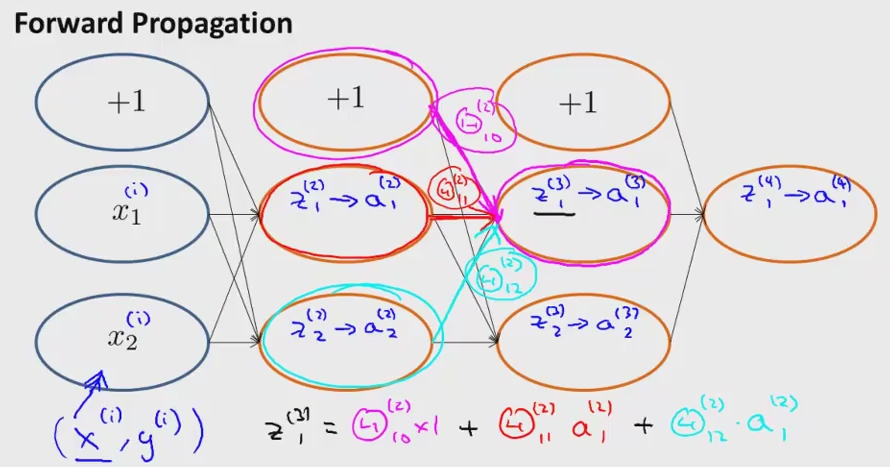
\includegraphics[scale=0.7]{sections/cs229/w6/forward_prop.png}
	\end{center}

	\item If you focus on a single example, the case of 1 output unit, and ignoring regularization ($\lambda = 0$): 
		$$\text{cost}(i)=y^{(i)}\log h(x^{(i)}) + (1-y{(i)} ) \log h(x^{(i)} )$$
	\item Formally, $\delta_j^{(l)}=\frac{\partial}{\partial z_j^{(l)}}\text{cost}(i)\text{ for } j\geq 0$
	\item Backpropagation looks identical, but backwards:
	\begin{center}
		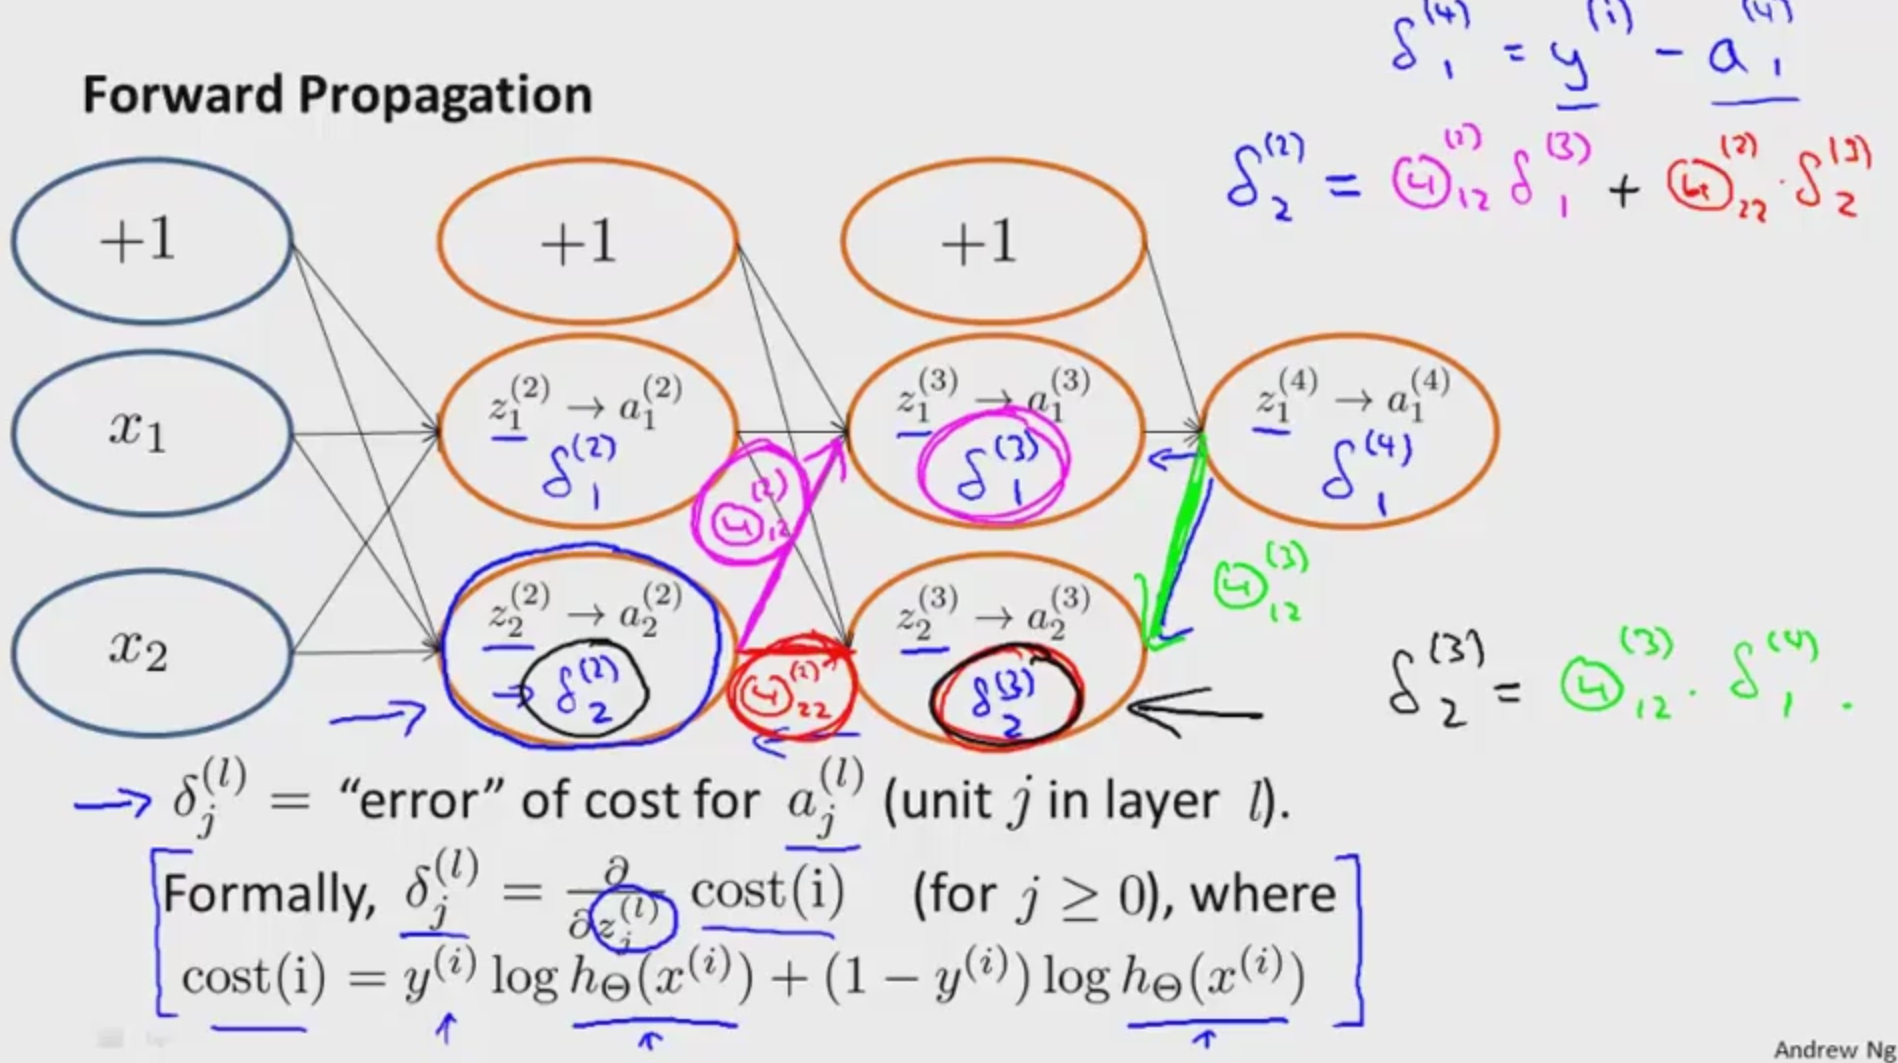
\includegraphics[scale=0.25]{sections/cs229/w6/back_prop.png}
	\end{center}
\end{itemize}

\subsubsection{Implementation Note: Unrolling Parameters}
\begin{itemize}[--]
	\item Our previous use of minfunc and costFunction in octave assumed that $\theta$ and the return would be vectors
	\item You can unroll elements into  large vector:
		thetaVec = [Theta1(:); Theta2(:); Theta3(:)];
	\item You can also change them back into the matrix using reshape:
		Theta1 = reshape(thetaVec(1:size),dim1, dim2);
	\begin{center}
		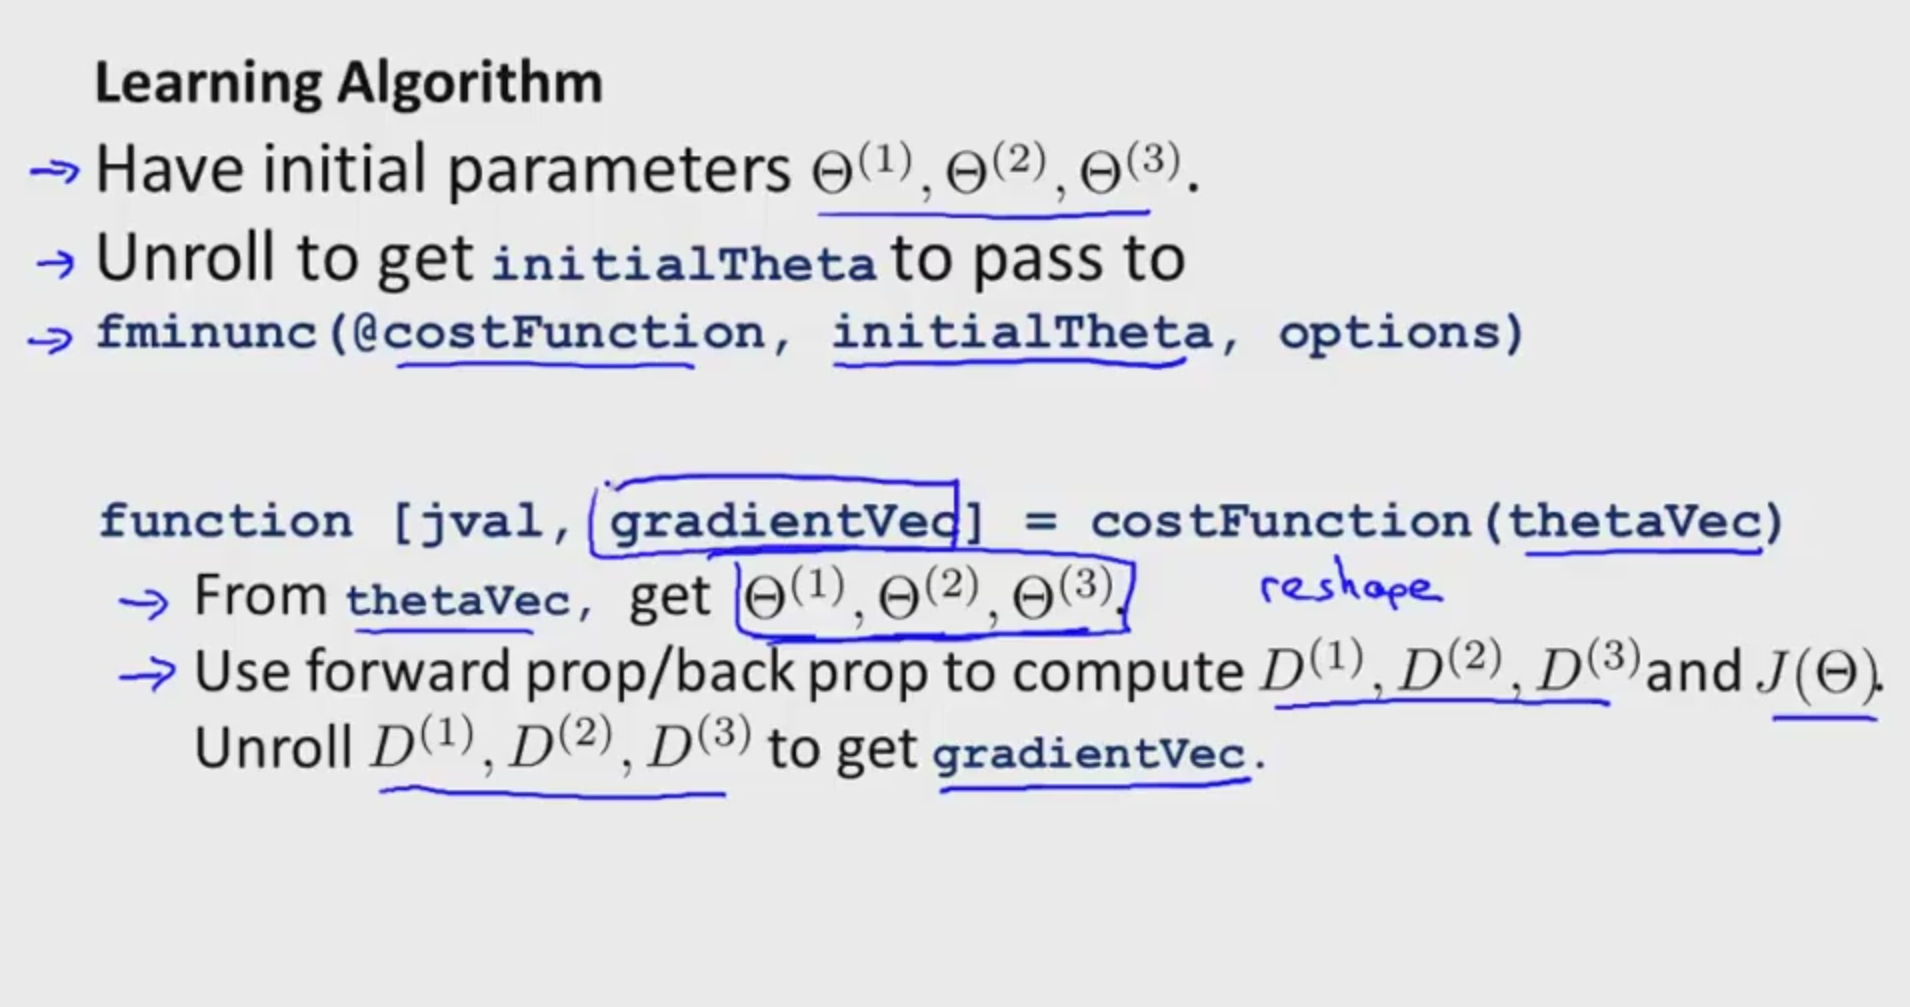
\includegraphics[scale=0.2]{sections/cs229/w6/algo.png}
	\end{center}
\end{itemize}

\subsubsection{Gradient Checking}
\begin{itemize}[--]
	\item Suppose you have a function $J(\Theta)$, and we want to estimate the derivative at $\theta\in\mathbb{R}$.
	\item We consider the points $\theta - \epsilon$ and $\theta + \epsilon$, and draw a line through these points and use the slope of this line as an approximation
	\item This gives our approximation as:
		$$\frac{d}{d\Theta} J(\Theta) = \frac{J(\Theta + \epsilon) - J(\Theta - \epsilon)}{2\epsilon}$$
	\item A good value for epsilon is: $\epsilon= 10^{-4}$
	\item Now consider $\theta\in\mathbb{R}^{n}$
	\item We can calculate the derivative for each element the same as we did for the single variable. Holding the other variables constant
	\item We then can compare this approximate derivative to the backpropagation to check that they're approximately the same
	\item Don't do gradient checking once you start learning, because it will be very slow
	\item j
\end{itemize}

\subsubsection{Random Initialization}
\begin{itemize}[--]
	\item Initializing all the parameters in a neural network, does not work like it did in our previous algorithms
	\item After each update, parameters corresponding to inputs going into each of two hidden units are identical
	\item This results in not being able to develop more complex features
	\item Instead, we will now initialize each $\Theta_{ij}^{(l)}$ to a random value in $\left[ -\epsilon, \epsilon \right]$
	\item The goal is ``symmetry breaking''
\end{itemize}

\subsubsection{Putting it Together}
\begin{itemize}[--]
	\item We must pick a network architecture (connectivity pattern between neurons)
	\item Reasonable default: 1 hidden layer, or if >1 hidden layer, have same number of hidden units in every layer (usually the more the better)
	\item Training a neural network:
	\begin{itemize}[--]
		\item Randomly initialize weights
		\item Implement forward propagation to get $h_{\Theta} (x^{(i)})$ for any $x^{(i)}$
		\item Impelement code to cmpute cost function $J(\Theta)$
		\item Implement backprop to compute partial derivatives $\frac{\partial}{\partial \Theta_{jk}^{(l)}} J(\Theta)$
		\item Perform forward propagation and backpropagation using each example
		\item Use gradient checking to compare partial derivatives computed using backpropagation vs. using numerical estimate of gradient of $J$. Then disable gradient checking code.
		\item Use gradient descent or advanced optimization method with backpropagation to try and minimize $J$ as a function of parameters $\Theta$
	\end{itemize}

	\item $J(\Theta )$ is non-convex, and can get stuck in local optimum
	
\end{itemize}

	\subsection{Advice for Applying Machine Learning}
	\subsubsection{Deciding What to Try Next}
\begin{itemize}[--]
	\item Suppose ou've trained your model, but it is largely error prone. What should you try next?
	\begin{itemize}[--]
		\item Get more training examples
		\item Try smaller sets of features
		\item Try getting additional features
		\item Try adding polynomial features
		\item Try decreasing $\lambda$
		\item Try increasing $\lambda$
	\end{itemize}

	\item \textbf{Diagnostic}: A test that you can run to gain insight what is/isn't working with a learning algorithm, and gain guidance as to how best to improve its performance
	\item Diagnostics can take time to implement, but oding so can be a very good use of your time
\end{itemize}

\subsubsection{Evaluating a Hypothesis}
\begin{itemize}[--]
	\item \textbf{Overfitting}: fails to generalize to new example not in training set
	\item How do we determine if it overfits?
	\item Suppose we have data set ${(x^{(i)}, y^{(i)} )}$, we will split the data into two sets: \textbf{training set}, and \textbf{test set}
	\item We will typically assign $~70\%$ to be the training set, and the remainder $~30\%$ to be the test set
	\item $m_{test}=$ number of test example
	\item Training/testing procedure for linear regression:
	\begin{itemize}[--]
		\item Learn parameter $\theta$ from training data (minimizing training error J($\theta$))
		\item Compute test set error:
			$$J_{test}(\theta_{training})=\frac{1}{2m_{test}}\sum_{i=1}^{m){test}}(h(x_{test}^{(i)}) - y_{test}^{(i)})^2$$
	\end{itemize} 

	\item Training/testing procedure for logistic regression:
	\begin{itemize}[--]
		\item Learn parameter $\theta$g from trainin data 
		\item Compute test set error:
			$$J_{test}(\theta_{training})=\frac{-1}{m_{test}}\sum_{i=1}^{m){test}}y_{test}^{(i)}\log h(x_{test}^{(i)}) + (1-y_{test}^{(i)}) \log h(x_{test}^{(i)} )$$
		\item Misclassification error (0/1 misclassification error):
			$$\text{err}(h(x), y)=\begin{cases}
				1 &\text{if } h(x)\geq 0.5 (y=0), \text{ or if } h(x)<0.5 (y=1)\\
				0 &\text{otherwise}
			\end{cases}$$
			$$\text{Test error} = \frac{1}{m_{test}}\sum_{i=1}^{m_{test}}\text{err}(h(x_{test}^{(i)}, y^{(i)})$$
	\end{itemize} 


\end{itemize}

\subsubsection{Model Selection and Train/Validation/Test Sets}
\begin{itemize}[--]
	\item If you consider adding another parameter to your model that is: $d=$degree of polynomial
		$$h(x;d)=\sum_{i=0}^{d}\theta_i x^{i}$$
	\item If we denote the parameters for each respctive model as $\theta^{(d)}$, we can then consider $J_{test}(\theta^{(d)}$ for each hypothesis
	\item Suppose we choose a model $\theta^{(5)}$, the problem with this system is it is likely to be an optimistic estimate of generalization error; namely, we fit the new parameter $d$ to the test set
	\item It is no longer fair to reuse the test set on this model to test it, because it's already favoring it
	\item Now we will split up the dataset into 3 pieces: \textbf{training set}, \textbf{cross validation set (cv)}, \textbf{test set}
	\item A typical split is 60\%-20\%-20\%, favoring the training set
	\item $m_{cv}=$ number of cross validation examples
	\item Training error:
		$$J_{train}(\theta) = \frac{1}{2m}\sum_{i=1}^{m} (h(x^{(i)}) - y^{(i)})^2$$
	\item Cross Validation error
		$$J_{cv}(\theta) = \frac{1}{2m_{cv}}\sum_{i=1}^{m_{cv}} (h(x^{(i)}_{cv}) - y^{(i)}_{cv})^2$$
	\item Test error
		$$J_{test}(\theta) = \frac{1}{2m_{test}}\sum_{i=1}^{m_{test}} (h(x^{(i)}_{test}) - y^{(i)}_{test})^2$$
	\item Now instead of the test set, we will use the cross validation set to select the model
	\item We will select the model based on the minimum of $J_{cv}(\theta^{(d)})$
	\item j

\end{itemize}


\subsubsection{Diagnosing Bias vs. Variance}
\begin{itemize}[--]
	\item Underfitting/overfitting problems
	\item Overfit = high variance
	\item Underfit = high bias
	\begin{center}
		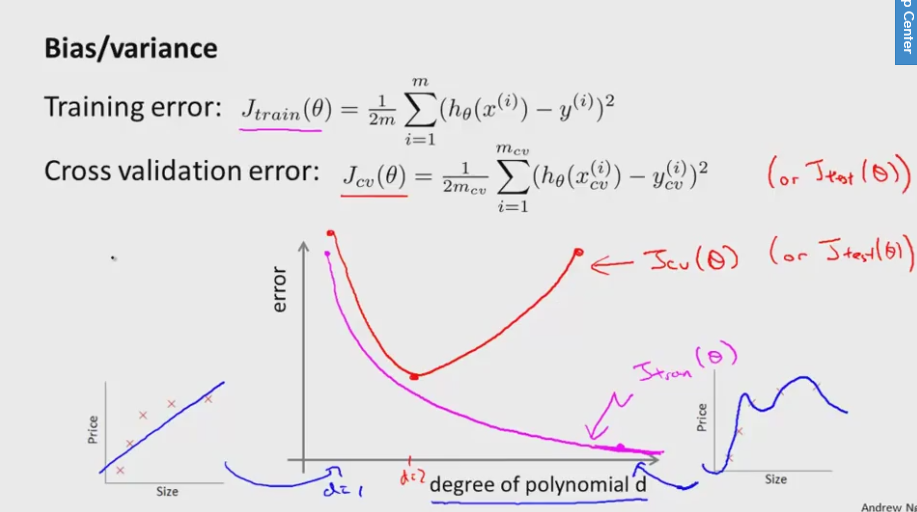
\includegraphics[scale=0.5]{sections/cs229/w7/bias_var.png}
	\end{center}

	\item High bias is shown on the left, where you have a low order polynomial with a large error
	\item High variance is shown on the right, where you have a high decree polynomial with a large error
	\item Your model suffers from high bias (underfit) problem if the training error is high and the cv is approximately the same.
	\item Your model suffers from high variance (overfit) if the training is low (fit well) while the cv error is much greater than the training error
\end{itemize}


\subsubsection{Regularization and Bias/Variance}
\begin{itemize}
	\item In regularization we have a regularization term with a variable $\lambda$
	\begin{center}
		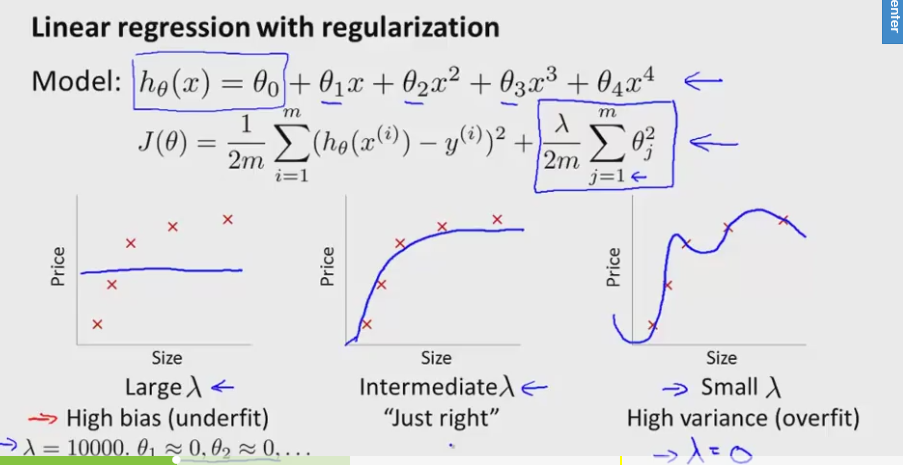
\includegraphics[scale=0.5]{sections/cs229/w7/reg.png}
	\end{center}

	\item When you have a large $\lambda$ all parameters are heavily penalized, so only the constant term remains
	\item Contrasting, when we have a small $\lambda$ we maintain our very high variance overfitting
	\item We want to find the ``just right'' value
	\item Choosing the regularization parameter $\lambda$
	\begin{itemize}
		\item Try multiples of $\lambda=0,0.01,0.02,0.04,0.08,\ldots, 10$
		\item Let the models of each value of $\lambda$ be $\theta^{(n)}$
		\item Choose the smallest $J_{cv}(\theta{(n)})$
	\end{itemize}

	\begin{center}
		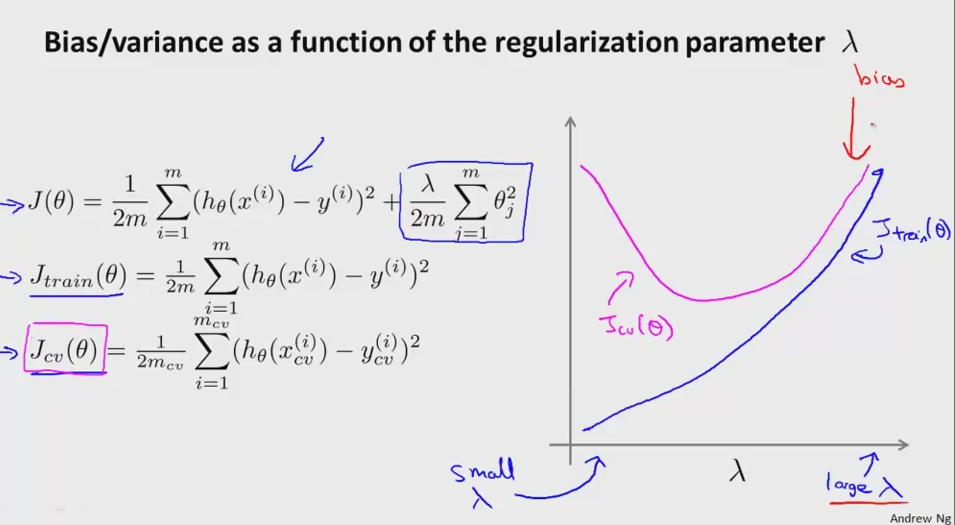
\includegraphics[scale=0.5]{sections/cs229/w7/lambda.png}
	\end{center}
	\item For small $\lambda$ you have little penalty and are able to fit your data well 
	\item The cross validation error is very high when $\lambda$ is small because you fit the too perfectly to other data set
\end{itemize}

\subsubsection{Learning Curves}
\begin{itemize}[--]
	\item Plot $J_{train}$ or $J_{cv}$ against $m$ (training set size)
	\item To do this we will deliberatly limit our training set size to complete the graph at lower points

	\item Suppose you have a high bais, If we were to increase the training set size you end up with a similar straight line
	\item The cv error will plateau out because the line can't conform any better to the data 
	\item The training set also has a similar error because it's unable to also conform to the data
	\item It has a high bias because both errors are high
	\item If a learning algorithm is suffering from high bias, getting more training data will not (by itself) help much.
	\begin{center}
		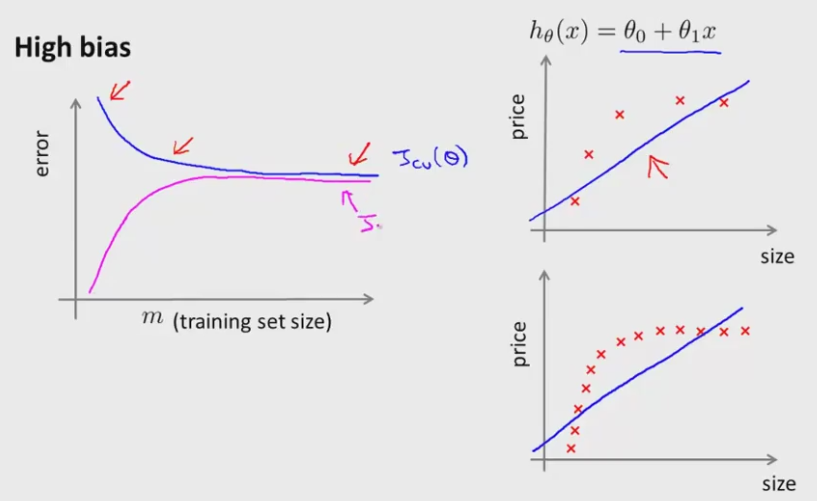
\includegraphics[scale=0.5]{sections/cs229/w7/bias.png}
	\end{center}

	\item Suppose now you have high variance, we will fit the data very well; however, it will largely overfit the data
	\item Since we can very easily fit the data our training error will remain low
	\item However, the cross validation error will remain high because it's too perfectly fitted for other data points
	\item The variance occurs do to this large gap in error between cv and training
	\item If a learning algorithm is suffering from high variance, getting more training data is likely to help.
	\begin{center}
		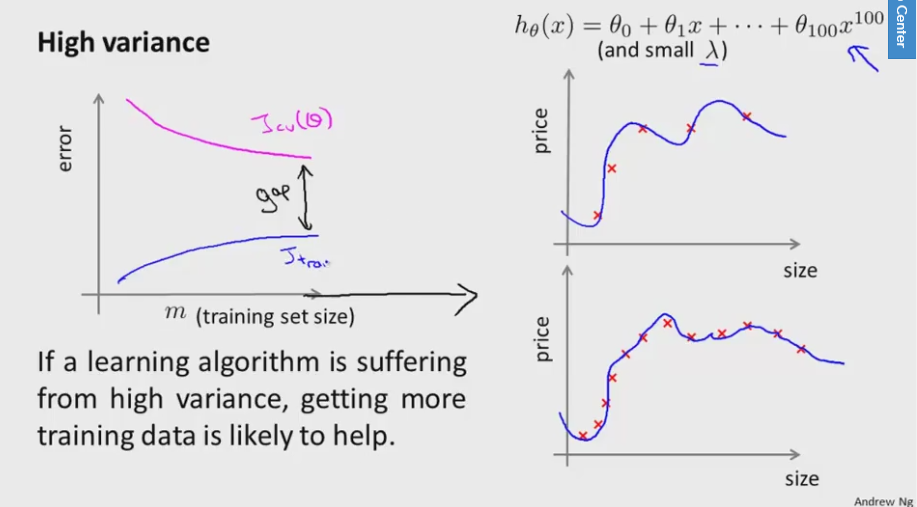
\includegraphics[scale=0.5]{sections/cs229/w7/var.png}
	\end{center}


\end{itemize} 

\subsubsection{Deciding What to Do Next Revisited}
\begin{itemize}[--]
	\item What should you try next?
	\begin{itemize}[--]
		\item Get more training examples $\to$ fixes high variance
		\item Try smaller sets of features  $\to$ fixes high variance
		\item Try getting additional features $\to$ fixes high bias (typically)
		\item Try adding polynomial features $\to$ fixes hih bias
		\item Try decreasing $\lambda$ $\to$ fixes high bias (less penalty for complex features)
		\item Try increasing $\lambda$ $\to$ fixes high variance (more penalty for complex features)
	\end{itemize}

	\item ``Small'' neural networks: fewer parameters; more prone to underfitting; computationally cheaper

	TODO: Draw

	\item ``Large'' neural network: more parameters; more prone to overfitting; computationally more expensive; use regularization to address overfitting

	TODO: Draw

	\item Try using the training/cv/test sets to determine the best choice for number of hidden layers
\end{itemize}


	\subsection{Machine Learning System Design}
	\subsubsection{Prioritizing What to Work On}
\begin{itemize}[--]
	\item Building a spam Classifier:
	\begin{itemize}[--]
		\item Supervised learning problem.
		\item $x=$features of email
		\item $y=$ spam (1) or not spam (0)
		\item Featurs $x$: choose 100 words indicative of spam/not spam
		\item $\vec{x}=$ 1 when the corresponding word appears, and 0 otherwise (eg. andrew is the first word, and it's in the email $x\left[ 0\right]=1$)
		\item Note: in practice, take most frequently occuring $n$ words (10000 to 50000) in training set, rather than manually pick 100 words
	\end{itemize}

	\item How to spend our time to make it have low error?
	\begin{itemize}[--]
		\item Collect lots of data
		\begin{itemize}[--]
			\item eg. ``honeypot'' project
		\end{itemize}

		\item Develop sophisticated features, for example based on email routing information (from email header)
		\item Develop sophisticated features for message body, eg. should ``discount'' and ``discounts'' be treated as the same word? How about ``deal'' and ``Dealer''? Features about punctuation?
		\item Develop sophisticated algorithm to detect misspellings (eg. m0rtgages, med1cine, w4tches)
	\end{itemize}
\end{itemize}

\subsubsection{Error Analysis}
\begin{itemize}[--]
	\item Recommended approach:
	\begin{itemize}
		\item Start with a simple algorithm that you can implement quickly. Implement it and test it on our cross-validation data
		\item Plot learning curves to decide if more data, more features, etc. are likely to help.
		\item Error analysis: Manually examine the examples (in cross validation set) that your algorithm made errors on. See if you spot any systematic trend in what type of examples it is making errors on
	\end{itemize}

	\item This allows evidence to decide our decisions, and not gut feelings
	\item Manually categorize errors when doing analysis:
	\begin{itemize}[--]
		\item What type of error is it
		\item What cues (features) you think would have helped the algorithm classify them correctly
	\end{itemize}

	\item The importance of numerical evaluation:
	\item Should discount/discounts/discounted/discounting be treated as the same word?
	\item Can use ``stemming'' software (eg. Porter stemmer)
	\item 
\end{itemize}

\subsubsection{Error Metrics for Skewed Classes}
\begin{itemize}[--]
	\item j
\end{itemize}

\subsubsection{Trading Off Precision and Recall}
\begin{itemize}[--]
	\item j
\end{itemize}

\subsubsection{Data For Machine Learning}
\begin{itemize}[--]
	\item j
\end{itemize}


% \section{Introduction and Overview}
% \section{Supervised Learning: Regression}
% \section{Supervised Learning: Classification}
% \section{Kernel Methods}
% \section{Regularization and Model Selection}
% \section{Advice on using ML Algorithms}
% \section{Neural Networks}
% \section{Unsupervised Learning}
% \section{Gaussian Process}
% \section{Ensemble Methods}
% \section{Sequence Modeling}
% \section{Learning Theory}

\end{document}